\documentclass[letterpaper,10pt,draftclsnofoot,onecolumn,titlepage]{IEEEtran}

\usepackage{graphicx}
\usepackage{amssymb}
\usepackage{amsmath}
\usepackage{amsthm}
\usepackage{alltt}
\usepackage{float}
\usepackage{color}
\usepackage{url}
\usepackage{enumitem}
\usepackage{pstricks, pst-node}
\usepackage{geometry}
\usepackage{array}


\geometry{margin = .75in}

\usepackage{hyperref}

\usepackage[acronym]{glossaries}

\makeglossaries

\newglossaryentry{iOS}{name={iOS}, description={A mobile operating system created and developed by Apple Inc. exclusively for Apple's hardware.}}

\newglossaryentry{ModelVC}{name={Model-View-Controller}, description={A design pattern that assigns objects in an application one of three roles: model, view, or controller. Also called MVC.}}

\newglossaryentry{Android}{name={Android}, description={A mobile operating system developed by Google, based on the Linux Kernel and designed primarily for touchscreen mobile devices.}}

\newglossaryentry{App}{name={app}, description={A software application designed to run on mobile devices such as smartphones or tablet computers.}}

\newacronym{ccb}{CCB}{Church Community Builder}

\newacronym{sdd}{SDD}{Software Design Document}

\newacronym{srs}{SRS}{Software Requirements Specification}

\newacronym{uml}{UML}{Unified Model Language}

\newacronym{mvc}{MVC}{Model-View-Controller}

\newacronym{xml}{XML}{EXtensible Markup Language}

\newacronym{ui}{UI}{User Interface}

\newcommand*{\signature}[1]{%
	\par\noindent\makebox[3.5in]{\hrulefill} \hfill\makebox[3.0in]{\hrulefill}%
	\par\noindent\makebox[3.5in][l]{#1}	    \hfill\makebox[3.0in][l]{Date}%
}%

\def\name{Kevin Stine, Courtney Bonn, Maxwell Dimm}
\def\team{Calvary Chapel Corvallis}
\def\grp{Group \#62}

\hypersetup{
	colorlinks = true,
	urlcolor = black,
	linkcolor = black,
	pdfauthor = {\name},
	pdftitle = {CS461 Design Document},
	pdfsubject = {CS461 Design Document},
	pdfpagemode = UseNone
}

\begin{document}
	\title{\huge \team \\ Design Document \\ CS 461 Fall 2016}
	\author{\large \name \\ \grp}



	\maketitle


		\begin{abstract}The purpose of this project is to produce an \gls{iOS} \gls{Android} \gls{App} for Calvary Chapel of Corvallis that will allow members to access a plethora of information all in one localized space.
		The Church's current website does not provide an interface where current members of the church can very quickly access important information such as events, bulletins, and messages from the service.
		The desired \gls{App} will be simple enough for anyone to use while providing back end access for staff to easily upload new information to the \gls{App}.
		The priorities lie in maximizing the usability of the \gls{App} and providing bulletin, schedule, video, and giving functionality.
		We will work with the existing Calvary Chapel web development team to create a product that is seamlessly integrated with their already existing network.
		\end{abstract}

	\section*{Signatures}

	\vspace{.5in}
	\signature{Client}
	\vspace{.5in}
	\signature{Courtney Bonn}
	\vspace{.5in}
	\signature{Kevin Stine}
	\vspace{.5in}
	\signature{Maxwell Dimm}


	\clearpage

	\tableofcontents

	\clearpage

	\section{Overview}

		\subsection{Scope}
			We will be implementing a mobile \gls{App} for both \gls{iOS} and \gls{Android} platforms.
			This \gls{App} will provide the members of Calvary Chapel Corvallis a centralized hub that will allow them to access the most important information about the church.
			Users will be able to view announcements, a calendar, e-bulletins, and sermons.
			Users will also be able to donate to the church.
			Three people will be involved in the implementation of this software and it will be done during October 2016 and June 2017.

		\subsection{Purpose}
			The purpose of this design document is to detail how the \gls{App} software will be designed.
			We will discuss how we will meet the requirements for our church \gls{App} and discuss the structure of the \gls{App}.
		\subsection{Intended Audience}
			The intended audience of this design document will be our clients, the teachers of CS 461, as well as the teacher's assistants.

		\printglossaries


	\section{Conceptual model for software design descriptions}

		\subsection{Software design descriptions within the life cycle}


			\subsubsection{Influences on \gls{sdd} preparation}
			\glsreset{sdd}
			\glsreset{srs}
				The key influence on this \gls{sdd} is the \gls{srs} document that has previously been documented.
				The requirements listed in the \gls{srs} will greatly determine the design of the software and how we implement this project.

			\subsubsection{Influences on software life cycle products}
				This \gls{sdd} may lead to necessary changes in the \gls{srs}.
				Throughout development, it's possible that there will be design changes that require us to change details in the \gls{srs}.
				Testing may also be changed based on the design document.

			\subsubsection{Design verification and design role in validation}
				In order to determine if the \gls{App} has met requirements, we will perform user testing.
				This will involve having users try to use the software in the intended manner and see if they are successful.
				Success will be determined by how many users are successfully able to use the \gls{App} without errors or issues.

	\section{Design description information content}

		\subsection{Introduction}
			Within this design document, there are many required contents.
			We will identify the \gls{sdd} and it's stakeholders.
			We will discuss design concerns and selected design viewpoints.
			We will also discuss design views, design overlays, and the design rationale.

		\subsection{\gls{sdd} Identification}
			A valid \gls{sdd} includes the following parts:
			\begin{itemize}
				\item{Date of issue and status}
				\item{Scope}
				\item{Issuing organization}
				\item{Authorship}
				\item{References}
				\item{Context}
				\item{One or more design languages for each design viewpoint used}
				\item{Body}
				\item{Summary}
				\item{Glossary}
				\item{Change history}
			\end{itemize}

		\subsection{Design stakeholders and their concerns}
			The design stakeholders of the Calvary Chapel of Corvallis \gls{App} are the developers of the app and the team at the church.
			Design concerns of the stakeholders include creating an \gls{App} that is user-friendly and very simplistic in design features.
			The final \gls{App} will be designed in a way that will ease this concern, as the intended design will be a very easy-to-use \gls{App}.

		\subsection{Design views}
		\glsreset{uml}
		We will use \gls{uml} diagrams in order to describe and represent the views of our system.

		\subsection{Design viewpoints}
		There are many viewpoints that will be covered in this document including: context, composition, logical, dependency, and interaction viewpoints.
		They each mean different things, for example the context viewpoint will cover what type of users will be using the \gls{App} and the perceptions they should have over it.
		The composition viewpoint will cover what information and content will be hosted within the \gls{App}.
		The logical viewpoint will cover what purpose the \gls{App} will serve and how it will accomplish those purposes.
		The dependency viewpoint will be the things the \gls{App} needs in order for it to work as designed and the integration of it with other \glspl{App}.
		Finally, we will conclude with the interaction viewpoint witch will cover how people will use our \gls{App} and how it will interact with various other technologies.

		\subsection{Design elements}
<<<<<<< HEAD
			Because the purpose of this design is to create a simplistic \gls{App} that will not require the user to do much searching, the elements we will incorporate into the design are somewhat simplistic as well.
			When the user opens the \gls{App}, the first thing she will see is a homepage that mimics their current website--white background with their logo at the top of the page.
			There will be a banner that is displayed which will frequently change and will be pulled from their website.
			There will be a menu with four buttons: messages, give, bulletin, and events.
			The menu will be available on each additional page.

			As far as design constraints go, this \gls{App} is going to be best suitable for current versions of both \gls{iOS} and \gls{Android} smartphones.
			For the \gls{iOS} \gls{App}, the screen resolution will be based off current screen sizes, approximately 4.7 inches and 5.5 inches (diagonal), though the \gls{App} will adjust to smaller and larger screens, allowing users to access the \gls{App} on older phone models as well as iPads.
			For the \gls{Android} \gls{App}, the screen resolution will adapt to all screen sizes, including tablets.

=======
			Because the purpose of this design is to create a simplistic app that will not require the user to do much searching, the elements we will incorporate into the design are somewhat simplistic as well.
			When the user opens the app, the first thing she will see is a homepage that mimics their current website--white background with their logo at the top of the page.
			There will be a banner that is displayed which will frequently change and will be pulled from their website.
			There will be a menu with four buttons: messages, give, bulletin, and events.
			The menu will be available on each additional page.

			As far as design constraints go, this application is going to be best suitable for current versions of both iOS and Android smartphones.
			For the iOS application, the screen resolution will be based off current screen sizes, approximately 4.7 inches and 5.5 inches (diagonal), though the app will adjust to smaller and larger screens, allowing users to access the app on older phone models as well as iPads.
			For the Android application, the screen resolution will adapt to all screen sizes, including tablets.

>>>>>>> master
		\subsection{Design overlays}
		When using the app we want to create a sense of continuity between the existing infrastructure and the app we are creating.
		We will be pulling the seasonal banner from the site purely as a stylistic decision.
		We will be keeping the color scheme simple, down to around 3 main colors matching those on their new unlisted website.
		The transition screen or loading screen for the app will be a simple black with the center being the Calvary Corvallis flame logo.
		This will also be used for the backdrop for our main pages of the app too but with the logo faded out as to not take away from the info on screen.
		Additionally we can create an overlay for the schedule and calendar that are simplistic and identify the information to the user such as a title at the top of the page.

		\subsection{Design rationale}
		Two of the primary focuses in our design rationale are to keep it simple for the users, and to keep is simple for the church management team.
		The client wants the \gls{App} to be as user friendly for the congregation at possible, along with keeping the back end work to a minimum.
		If the \gls{App} is too confusing for the users or the team, then the whole purpose of this \gls{App} will be voided by their inability to use it.
		Secondary to these points is maximizing speed and adding additional small features.
		We should be creating an efficient \gls{App} that can have helpful functionality for the users.

		\subsection{Design languages}
		The design language that we will use in this document will be \gls{uml}.

	\section{Design Viewpoints}

		\subsection{Introduction}
		In this section, we will discuss seven design viewpoints including:
			\begin{itemize}
				\item{Context Viewpoint}
				\item{Composition Viewpoint}
				\item{Logical Viewpoint}
				\item{Dependency Viewpoint}
				\item{Patterns Use Viewpoint}
				\item{Interface Viewpoint}
				\item{Interaction Viewpoint}
			\end{itemize}

		\subsection{Context Viewpoint}
		Included in the \gls{App} are four primary functionalities: calendar, sermons, donations, and bulletin.
		The reason being is that these are the four primary things that our client believes their users will be looking to access from the \gls{App}.
		The schedule will be there to allow users to see what is going on within the church in the long-term.
		The sermon functionality will allow people to view past sermons in case they missed them or simply want to recap a message they enjoyed.
		In this church and many others donating is a major part of what they do.
		Making this easier for the users of our \gls{App} is crucial.
		Now they can do it from home or any time because the \gls{App} will allow them to give without the need of cash on hand.
		Finally the last functionality that we want to include is the bulletin.
		This will be a place for the users to grab quick info that would normally be handed out on a piece of paper inside the building.
		his will allow them to view the bulletin from anywhere at any time and reduce costs for the church to prevent the need of printing off pamphlets.

		\begin{figure}[H]
			\centering
			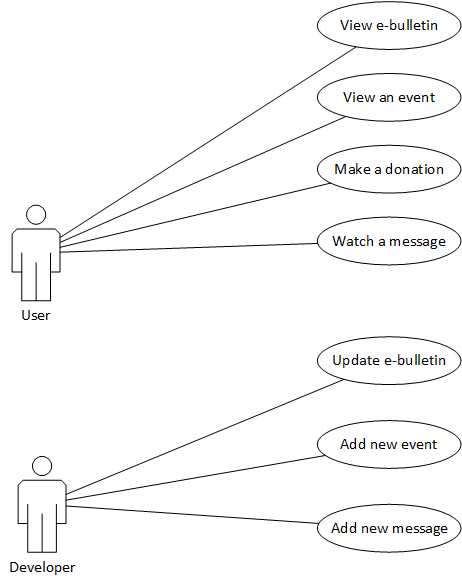
\includegraphics[natwidth=462, natheight=585]{UseCase.png}
			\caption{Use Case Diagram}
			\label{fig:usecase}
		\end{figure}


		\subsection{Composition Viewpoint}
		\glsreset{ccb}
			Our system is composed of four components which are an \gls{iOS} Client, an \gls{Android} Client, a Database Server and a Web Server.
			The Database Server which we connect to is through \gls{ccb}.
			The Web Server which we connect to is Calvary Chapel's current website.
			Client components are comprised of smartphone \glspl{App}, based on their operating system.
			Our \gls{iOS} and \gls{Android} Clients will be able to pull information from both CCB as well as the church's current website.

		\begin{figure}[H]
			\centering
			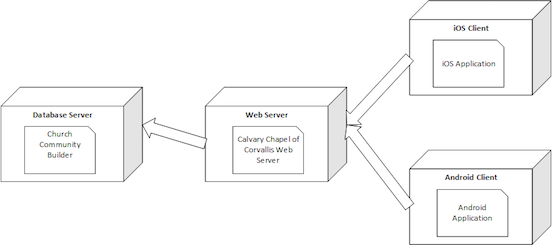
\includegraphics[natwidth=552, natheight=245]{Deployment.png}
			\caption{Deployment Diagram}
			\label{fig:deployment}
		\end{figure}

		\subsection{Logical Viewpoint}
			There will be four main classes which make up the bulk of this \gls{App}.
			These classes include: events, messages, donations, and the bulletin.
			In this section, we will describe the details of what each class will do.

			\subsubsection{Events Class}
				The events class will handle pulling the calendar from the church's database and displaying it on the \gls{App} for the user to see.
				The adding and updating of events will be handled by the staff on the database, \gls{ccb}.
				All changes will then be pushed to the \gls{App}.

			\subsubsection{Messages}
				The messages class will handle displaying the recent sermon in either video or audio form.
				The video will be pulled from the church's existing system, LiveStream.

			\subsubsection{Donations}
				The donations class will handle the interface for users to make a donation to the church.
				We will connect this page to the church's existing donation system, Authorize.net, which will allows the users to make a secure donation.

			\subsubsection{Bulletins}
				The bulletins class will handle displaying the current bulletin on the \gls{App}.
				The bulletin will be pulled from the database, \gls{ccb}, and displayed on the \gls{App}.
				In order to update the bulletin, the staff at Calvary Chapel of Corvallis will update the information on their database, which will push the changes to the \gls{App}.

		\subsection{Dependency Viewpoint}
			The \gls{App} will have a couple interconnections with other \glspl{App} plugins.
			The first and foremost will be with \gls{ccb}.
			Most of the information we will be pulling from continuously will be from CCB, such as the schedule and bulletin.
			Also we will need to work with LiveStream's API to get a functional video/audio player for the sermons section.
			Our client already uses foxycart for their donation service so we will integrate their service to our \gls{App} using their published API.
			We will be sending information to their servers so we will also need to find a way to encrypt the data being sent because it is highly personal info.

		\subsection{Patterns use viewpoint}
		\glsreset{mvc}
			Our system will make use of the \gls{ModelVC} \gls{Android} design pattern.
			The \gls{mvc} design pattern assigns objects in an \gls{App} with one of three roles: model, view or controller.
			In addition to defining the roles the objects play in the \gls{App}, it also defines the way objects communicate with each other.
			For example when the user refreshes the sermons page to get the latest sermons, the model object changes and notifies the controller object which will then update the sermons view objects.

			\subsubsection{Model Objects}
			\glsreset{xml}
				Model objects encapsulate the data specific to the \gls{App} and define the logic and computation that manipulate and process the data.
				In our \gls{App}, there will be data specific to donations, calendar, e-bulletins and messages.
				This will strictly be the data that we pull from the CCB database and the Church's website and will not be concerned with user-interface and presentation issues.
				We will parse the CCB information as \gls{xml} and read that into our \gls{App} as \gls{xml}.
				The model object will strictly deal with data pulled from the CCB database.
				Once the data has been retrieved, it will notify the controller object to begin the process of updating the user's view.
				This object is hidden via an abstraction layer, ensuring that the user is only able to view the information we provide them in a clean and concise view.

			\subsubsection{View Objects}
			\glsreset{ui}
				The view object is an object in an \gls{App} that the users can see.
				Our \gls{App} will utilize the view objects to display data from our model object which is pulled from CCB.
				This object is what the user will see and interact with through our \gls{App}.
				View objects will be consistent across pages to ensure the most navigable \gls{ui} for the user.
				An example of the view object would be when the user wants to view the calendar for events.
				If they are in the month of December and want to look ahead to January, they will tap to proceed to the next month, which will notify the controller object letting the model object know to pull January's data from the database.

			\subsubsection{Controller Objects}
				The controller object will act as an intermediary between our \gls{App} views and its model objects.
				The controller will be a conduit through which view objects learn about changes in model objects and vice versa.
				In addition to communication between the view and model objects, the controller object will also perform setup, coordinate tasks and manage the life cycle of other objects.
				When the model object is updated with the month of January, the controller object communicates the new data to the view objects so they can be displayed to the user.


		\subsection{Interface viewpoint}
			Our system will utilize tabbed applications to allow for easy navigation through the pages.
			For both \gls{iOS} and \gls{Android}, we will have persistent buttons at the bottom of the screen giving the user an efficient and discoverable navigation pane.
			This allows for the most discoverability, as the user can interact with each page directly from the home page by clicking any of the icons at the bottom of the screen.
			Rather than having the user swipe in from the side to access a side bar menu, we want to give the users a consistent view across platforms that it easily recognizable.
			By tapping on a bottom navigation icon, the user will be directly taken to that associated view, or have the currently active page refreshed.

			Our application will make use of the following five navigable options:
			\begin{itemize}
				\item \textbf{Home:} The main page that users will see when they open the application. Should show some basic data pulled from either CCB or the website such as the logo, banner, and potentially any updates/news.
				\item \textbf{Events:} The events page will show the user a calendar view that will get pulled down from the CCB database.
				\item \textbf{Bulletin:} The page to allow the user to view updates and announcements in the form of a bulletin. Will pull the bulletin from the CCB database and pushed to the view object.
				\item \textbf{Donate:} The page to allow users to donate to the church. We will link in directly to the Church's donation vendor (Foxycart) and utilize their API to make calls when users want to donate.
					Our fallback method will be to utilize an in-app browser that will bring the user to the donation page.
				\item \textbf{Sermons:} This page will bring up the past sermons from the Church's Database, either through CCB or a third party site such as livestream or YouTube..
					This is still under discussion, however if the sermons are uploaded to CCB, we can just pull those in from the database and display them using the respective built-in video players.
					If the Church decides to use a different platform such as YouTube
			\end{itemize}

			A tabbed application is a built-in layout for Xcode and will be utilized through Apple's Interface Builder.
			Through the Interface Builder we will make use of the following storyboard controllers:
			\begin{itemize}
				\item Table View Controller
				\item Navigation Controller
				\item Tab Bar Controller
			\end{itemize}
			We will add relationships between the initial storyboard view and the other tab pages, to allow for smooth transitions between various pages.

		\subsection{Interaction Viewpoint}
			The Interaction viewpoint describes the high-level functionality of each part of the \gls{App}.
			There are four different functionalities that will be addressed: viewing the calendar, reading the bulletin, donating to the church, and watching the message.

			\subsubsection{Viewing the Calendar}
				\begin{enumerate}
					\item \textbf{Open \Gls{App}:} The interaction begins with the user open the \gls{iOS} or \gls{Android} \gls{App}.
					\item \textbf{Click Calendar:} After opening the \gls{App}, the user will see the menu and choose the option to view the calendar.
					\item \textbf{Pull Calendar:} Once the user has clicked on the calendar, the \gls{App} will fetch the calendar from the database, \gls{ccb}.
					\item \textbf{Return and Display Calendar:} The database will then display the calendar on the \gls{App}.
				\end{enumerate}

			\subsubsection{Reading the Bulletin}
				\begin{enumerate}
					\item \textbf{Open \Gls{App}:} The interaction begins with the user open the \gls{iOS} or \gls{Android} \gls{App}.
					\item \textbf{Click Bulletin:} After opening the \gls{App}, the user will see the menu and choose the option to open the bulletin.
					\item \textbf{Pull Bulletin:} Once the user has clicked on the bulletin, the \gls{App} will fetch the e-bulletin from the database, \gls{ccb}.
					\item \textbf{Return and Display Bulletin:} The database will then display the e-bulletin on the \gls{App}.
				\end{enumerate}

			\subsubsection{Donating to the Church}
				\begin{enumerate}
					\item \textbf{Open \Gls{App}:} The interaction begins with the user open the \gls{iOS} or \gls{Android} \gls{App}.
					\item \textbf{Click Bulletin:} After opening the \gls{App}, the user will see the menu and choose the option to donate.
					\item \textbf{Load Donation Page:} Once the user has clicked on the donate button, a page will load that will connect the user to Calvary Chapel of Corvallis' webpage that will display the donation page.
					The user will then follow the instructions on the page to continue making a donation to the church.
				\end{enumerate}

			\subsubsection{Watching the Message}
				\begin{enumerate}
					\item \textbf{Open \Gls{App}:} The interaction begins with the user open the \gls{iOS} or \gls{Android} \gls{App}.
					\item \textbf{Click Messages:} After opening the \gls{App}, the user will see the menu and choose the option to open the messages.
					\item \textbf{Pull Messages:} Once the user has clicked on the messages, the \gls{App} will fetch the message from LiveStream.
					\item \textbf{Return and Display Message:} LiveStream will then display the recent video message.
				\end{enumerate}




	\section{Conclusion}
	\glsreset{ccb}
		The \gls{App} we are building is a very user-friendly, simple app that will allow the members of the Calvary Chapel of Corvallis to access the most important pieces of their main website.
		This design document describes how our system for the \gls{App} is going to work.
		It details the different parts of the system and how they will interact with each other.
		Additionally it describes how each part will work with the church's database, \gls{ccb}.
		The design document provides a design framework for how the \gls{App} is going to be implemented and will continue to change depending on the implementation of the project.


\end{document}
